% --------------------------------------------------------------
% This is all preamble stuff that you don't have to worry about.
% Head down to where it says "Start here"
% --------------------------------------------------------------
 
\documentclass[12pt]{article}
 
\usepackage[margin=1in]{geometry} 
\usepackage{amsmath,amsthm,amssymb,mathtools}
\usepackage{dsfont} % for indicator function \mathds 1
\usepackage{tikz,pgf,pgfplots}
\usepackage{enumerate} 
\usepackage{graphicx,float} % figures

\newenvironment{theorem}[2][Theorem:]{\begin{trivlist} %% Theorem Environment
\item[\hskip \labelsep {\bfseries #1}\hskip \labelsep {\bfseries #2.}]}{\end{trivlist}}

\newtheorem{definition}{Definition}
\let\olddefinition\definition
\renewcommand{\definition}{\olddefinition\normalfont}
\newtheorem{lemma}{Lemma}
\let\oldlemma\lemma
\renewcommand{\lemma}{\oldlemma\normalfont}
\newtheorem{proposition}{Proposition}
\let\oldproposition\proposition
\renewcommand{\proposition}{\oldproposition\normalfont}
\newtheorem{corollary}{Corollary}
\let\oldcorollary\corollary
\renewcommand{\corollary}{\oldcorollary\normalfont}

\newcommand\norm[1]{\left\lVert#1\right\rVert} % \norm command 


%% set some plotting parameters in tikz & pgfplots
\usetikzlibrary{patterns}


\pgfmathsetseed{26} % for Brownian Motion plotting
\newcommand{\Emmett}[5]{% points, advance, rand factor, options, end label
\draw[#4] (0,0)
\foreach \x in {1,...,#1}
{   -- ++(#2,rand*#3+0.001)
}
node[right] {#5};
}
\pgfplotsset{every axis/.append style={},
    cmhplot/.style={mark=none,line width=1pt,->},
    soldot/.style={only marks,mark=*},
    holdot/.style={fill=white,only marks,mark=*},
    soldotSQ/.style={only marks,mark=square*},
    holdotSQ/.style={fill=white,only marks,mark=square*},
    soldotTR/.style={only marks,mark=triangle*,mark options={scale=1.5}},
    holdotTR/.style={fill=white,only marks,mark=triangle*,mark options={scale=1.5}},
}

%% set noindent by default and define indent to be the standard indent length
\newlength\tindent
\setlength{\tindent}{\parindent}
\setlength{\parindent}{0pt}
\renewcommand{\indent}{\hspace*{\tindent}}

\begin{document}

% --------------------------------------------------------------
%                         Start here
% --------------------------------------------------------------
 
\title{Mathematical \& Computational Finance II\\Lecture Notes}
\author{Introduction to Stochastic Calculus}
\date{September 29 2015 \\ Last update: \today{}}
\maketitle

%% SECTION: STOCHASTIC INTEGRALS
\begin{section}{Stochastic Integrals}
\indent Last time we discussed the quadratic variation of Brownian Motion and why that means its interesting. Now, we elaborate and move onto stochastic integration.

\begin{definition} A \underline{simple process} $H$ from $[0,T]\times\Omega \rightarrow \mathbb R$ is such that\footnote{For It\^{o} integrals we require that our processes be ``right continuous'', i.e. we have $t \in (t_i, t_{i + 1}]$.}
\begin{equation*}
	H_t(\omega) = 
		\begin{cases}
			H_0(\omega) & t \in (t_0, t_1] \\
			H_{t_i}(\omega) & t \in (t_i, t_{i+1}]
		\end{cases}
\end{equation*}
with partition $0 = t_0 \leq \cdots \leq t_N = T$ of $[0,T]$ where $H_{t_i}$ is $\mathcal F_{t_i}$-measurable (i.e. it's a random variable).

\begin{figure}[h!]
\centering
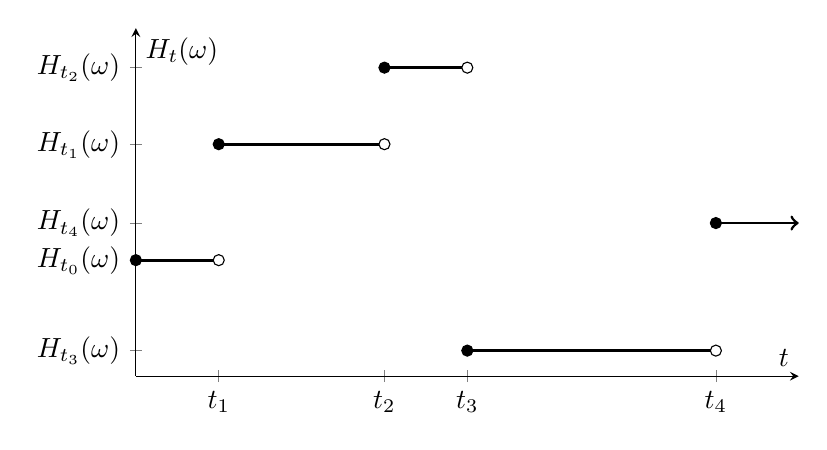
\begin{tikzpicture}
\begin{axis}
	[
		height 		= 6cm,
		width		 	= 10cm,
		axis line style	= {->}, % arrows on the axis
		xmin			= -0,
		xmax			= 8,
		xtick 			= {1,3,4,7},
		xticklabels 		= {$t_1$,$t_2$,$t_3$,$t_4$},
		xlabel		= {$t$},          % default put x on x-axis
		axis x line		= middle,    % put the x axis in the middle
            	ymin			= 0,
		ymax			= 1.5,
		ylabel		= {$H_t(\omega)$},          % default put y on y-axis
		axis y line 		= middle,    % put the y axis in the middle
		yticklabels 		= {$H_{t_0}(\omega)$,$H_{t_1}(\omega)$,$H_{t_2}(\omega)$,$H_{t_3}(\omega)$,$H_{t_4}(\omega)$},
		ytick			= {0.5,1,1.33,0.11,0.66},
        ]
	\addplot[soldot]coordinates{(0,0.5)(1,1)(3,1.33)(4,0.11)(7,0.66)};
	\addplot[holdot]coordinates{(1,0.5)(3,1)(4,1.33)(7,0.11)};
       	\addplot[cmhplot,-,domain=0:1]{0.5};
         \addplot[cmhplot,-,domain=1:3]{1};
        	\addplot[cmhplot,-,domain=3:4]{1.33};
        	\addplot[cmhplot,-,domain=4:7]{0.11};
	\addplot[cmhplot,->,domain=7:8]{0.66};
\end{axis}
\end{tikzpicture}
\end{figure}
\end{definition}

\begin{definition} Let $t \in [0,T]$ and consider the partition $0 = t_0 < t_1 < \cdots < t_m = T$. Suppose that $H \in \mathcal H_T$ is a simple process with representation
\begin{equation*}
	H_t(\omega) =
	\begin{cases}
		H_0(\omega) & t \in (t_0, t_1] \\
		H_{t_i}(\omega) & \text{if } t \in (t_i, t_{i + 1}]
	\end{cases}
\end{equation*}

with respect to Brownian Motion $B_t$ on a filtered probability space $(\Omega, \mathcal F, (\mathcal F_t)_{t\geq0},\mathbb P)$. Consider some random variables $\left\{ H_{t_i} \right\}^m_{i = 0}$ such that each $H_{t_i}$ is $\mathcal F_{t_i}$-measurable and bounded. We define the \underline{stochastic integral} (It\^{o} integral) with respect to the Brownian motion $B_t$ as
\begin{equation*}
	W(T) = \int^T_0 H_u \,dB_u
\end{equation*}

\end{definition}

%% SUBSECTION: PROPERTIES
\subsection{Properties}
\noindent For simple processes $H$ and $K$ and constants $\alpha, \beta$
\begin{enumerate}
	\item Linearity: $\int^t_0 (\alpha H_u + \beta K_u)\,dB_u = \alpha\int^t_0 H_u\,dB_u + \beta\int^t_0 K_u\,dB_u$
	\item $W(t) = \int^t_0 H_u\,dB_u$ is a martingale.
	\item $\mathbb E[(W(t))^2] = \mathbb E[(\int^t_0 H_u\,dB_u)^2] = \mathbb E[\int^t_0 H^2_u\,du]$
\end{enumerate}

\indent For some visual intuition of the ``simple proof'' that integrals of simple processes are linear, let $X_t = H_t + K_t$ then we can see the following
\vspace{5pt}
\begin{figure}[h!]
\centering
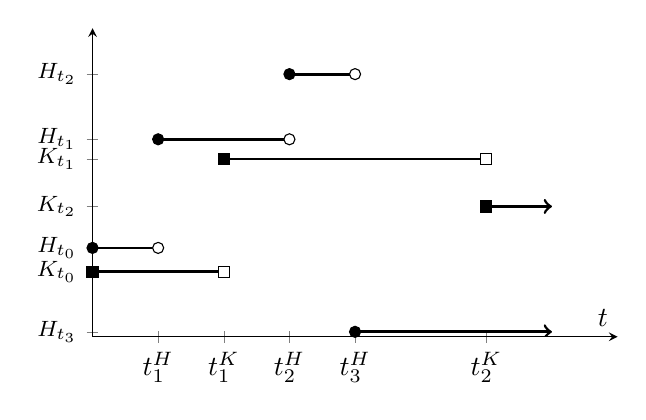
\begin{tikzpicture}
\begin{axis}
	[
		height 		= 5.5cm,
		width		 	= 8.25cm,
		axis line style	= {->}, % arrows on the axis
		xmin			= -0,
		xmax			= 8,
		xtick 			= {1,2,3,4,6},
		xticklabels 		= {$t_1^H$,$t^K_1$,$t^H_2$,$t^H_3$,$t^K_2$},
		xlabel near ticks,
		xlabel		= {$t$},          % default put x on x-axis
		axis x line		= middle,    % put the x axis in the middle
            	ymin			= 0,
		ymax			= 1.5625 ,
		ylabel		= {},          % default put y on y-axis
		axis y line 		= middle,    % put the y axis in the middle
		yticklabels 		= {\footnotesize{$H_{t_0}$},\footnotesize{$H_{t_1}$},\footnotesize{$H_{t_2}$},\footnotesize{$H_{t_3}$},\footnotesize{$K_{t_0}$},\footnotesize{$K_{t_1}$},\footnotesize{$K_{t_2}$}},
		ytick			= {0.45,1,1.33,0.025,0.33,0.9,0.66}
        ]
	\addplot[soldot]coordinates{(0,0.45)(1,1)(3,1.33)(4,0.025)};
	\addplot[holdot]coordinates{(1,0.45)(3,1)(4,1.33)};
       	\addplot[cmhplot,-,domain=0:1]{0.45};
         \addplot[cmhplot,-,domain=1:3]{1};
        	\addplot[cmhplot,-,domain=3:4]{1.33};
        	\addplot[cmhplot,->,domain=4:7]{0.025};
	\addplot[soldotSQ] coordinates {(0,0.33)(2,0.9)(6,0.66)};
	\addplot[holdotSQ] coordinates {(2,0.33)(6,0.9)};
        	\addplot[cmhplot,-,domain=0:2]{0.33};
        	\addplot[cmhplot,-,domain=2:6]{0.9};
        	\addplot[cmhplot,->,domain=6:7]{0.66};
\end{axis}
\end{tikzpicture}
\begin{tikzpicture}
\begin{axis}
	[
		height 		= 8cm,
		width		 	= 8.25cm,
		axis line style	= {->}, % arrows on the axis
		xmin			= -0,
		xmax			= 8,
		xtick 			= {1,2,3,4,6},
		xticklabels 		= {$t_1^*$,$t_2^*$,$t_3^*$,$t_4^*$,$t_5^*$},
		xlabel near ticks,
		xlabel		= {$t$},          % default put x on x-axis
		axis x line		= middle,    % put the x axis in the middle
            	ymin			= 0,
		ymax			= 2.5,
		ylabel		= {},          % default put y on y-axis
		axis y line 		= middle,    % put the y axis in the middle
		yticklabels 		= {\footnotesize{$X_{t_0}$},\footnotesize{$X_{t_1}$},\footnotesize{$X_{t_2}$},\footnotesize{$X_{t_3}$},\footnotesize{$X_{t_4}$},\footnotesize{$X_{t_5}$}},
		ytick			= {0.78,1.33,1.9,2.23,0.88,0.685}
        ]
	\addplot[soldotTR] coordinates{(0,0.78)(1,1.33)(2,1.9)(3,2.23)(4,0.88)(6,0.685)};
	\addplot[holdotTR] coordinates{(1,0.78)(2,1.33)(3,1.9)(4,2.23)(6,0.88)};
	\addplot[cmhplot,-,domain=0:1]{0.78};
       	\addplot[cmhplot,-,domain=1:2]{1.33};
	\addplot[cmhplot,-,domain=2:3]{1.9};
	\addplot[cmhplot,-,domain=3:4]{2.23};
	\addplot[cmhplot,-,domain=4:6]{0.88};
	\addplot[cmhplot,->,domain=6:7]{0.685};
\end{axis}
\end{tikzpicture}
\caption{By combining the existing partitions of $H$ and $K$ we can produce a new simple process which has the value of $X_t = H_t + K_t$ at every point $t$ defined for $H$ and $K$. Clearly we see that scaling $H$ and $K$ by constants $\alpha,\beta$ produces an analoguous result.}
\end{figure}

\begin{proof} {\em Proof that $W(t) = \int^t_0 H_u\,dB_u$ is a martingale}. By assumption there exists a partition $0 = t_0 \leq \cdots \leq t_N = T$ such that
\begin{equation*}
	H_t(\omega) = 
		\begin{cases}
			H_0(\omega) & t \in (t_0, t_1] \\
			H_{t_i}(\omega) & t \in (t_i, t_{i+1}]
		\end{cases}
\end{equation*}

where $H_{t_i} \in \mathcal F_{t_i}$. Suppose $t \in (t_k, t_{k+1}]$ then,
\begin{equation*}
	W(t) = H_{t_k}(B_t - B_{t_k}) + \sum^k_{i = 1} H_{t_{i-1}} (B_{t_i} - B_{t_{i-1}})
\end{equation*}

\indent To complete the proof we must show that $W(t)$ is $\mathcal F_t$-measurable, integrable, and satisfies the martingale property: $\mathbb E[W(t)|\mathcal F_s] = W(s)$. Clearly $W(t)$ is $\mathcal F_t$-measurable since its components
\begin{align*}
	H_{t_{i-1}} &\in \mathcal F_{t_{i-1}} \subset \mathcal F_t \quad \text{and} \\
	(B_{t_i} - B_{t_{i-1}}) &\in \mathcal F_{t_i} \subset \mathcal F_t \quad \text{and} \\
	H_{t_k} &\in \mathcal F_{t_k} \subset \mathcal F_t \quad \text{and} \\
	(B_t - B_{t_k}) &\in \mathcal F_{t_k} \subset \mathcal F_t
\end{align*}

\indent So every component of $W(t)$ is $\mathcal F_t$-measuable and a sum/product of $\mathcal F_t$-measurable elements is itself $\mathcal F_t$-measurable.\footnote{Is this statement obvious?}~\footnote{I think we skip the integrability condition and move on directly to the martingale property.}~For $0 \leq s < t$ and $s \in (t_j, t_{j+1}]$ for $j < k$, thus $s < t$, we have
\begin{align*}
	\mathbb E[W(t)|\mathcal F_s] &= \mathbb E[ H_{t_k}(B_t - B_{t_k}) + \sum^k_{i = 1} H_{t_{i-1}} (B_{t_i} - B_{t_{i-1}})|\mathcal F_s] \\
	&= \mathbb E[H_{t_k}(B_t - B_{t_k})|\mathcal F_s]  + \mathbb E[\sum^k_{i = 1} H_{t_{i-1}} (B_{t_i} - B_{t_{i-1}})|\mathcal F_s]
\end{align*}

But notice
\begin{align*}
	\mathbb E[H_{t_k}(B_t - B_{t_k})|\mathcal F_s] &= \mathbb E[\mathbb E[H_{t_k}(B_t - B_{t_k})|\mathcal F_{t_k}]|\mathcal F_s] \quad \text{(by the tower property)} \\ 
	&= \mathbb E[H_{t_k} \mathbb E[B_t - B_{t_k}|\mathcal F_{t_k}]|\mathcal F_s] \quad \text{(taking out what's known)}\\
	&= \mathbb E[H_{t_k}\cdot 0 |\mathcal F_s] = 0 \quad \text{(by independent increments with mean 0)}
\end{align*}

So we're left with
\begin{align*}
	\mathbb E[W(t)|\mathcal F_s] &= 0 + \mathbb E[\sum^k_{i = 1} H_{t_{i-1}} (B_{t_i} - B_{t_{i-1}})|\mathcal F_s]\\
	&=  \mathbb E[\sum^j_{i = 1} H_{t_{i-1}} (B_{t_i} - B_{t_{i-1}}) + H_{t_{j}} (B_{s} - B_{t_{j}}) + H_{s} (B_{t_{j+1}} - B_{t_{j}}) + \\
	&\hphantom{{}=\mathbb E[\sum^j_{i = 1} H_{t_{i-1}} (B_{t_i} - B_{t_{i-1}}) + H_{t_{j}} (B_{s}} \sum^k_{i = j + 2} H_{t_{i-1}} (B_{t_i} - B_{t_{i-1}})|\mathcal F_s] \\
	&= \mathbb E[W(s) + H_{s} (B_{t_{j+1}} - B_{t_{j}}) + \sum^k_{i = j + 2} H_{t_{i-1}} (B_{t_i} - B_{t_{i-1}})|\mathcal F_s]  \\
	&= W(s) + H_s\mathbb E[B_{t_{j+1}} - B_{t_{j}}|\mathcal F_s] + \mathbb E[\sum^k_{i = j + 2} H_{t_{i-1}} (B_{t_i} - B_{t_{i-1}})|\mathcal F_s] \\
	&= W(s) + H_s\cdot0 + \mathbb E[\sum^k_{i = j + 2} H_{t_{i-1}} (B_{t_i} - B_{t_{i-1}})|\mathcal F_s] \\
	&=  W(s) + \sum^k_{i = j + 2} \mathbb E[\mathbb E[H_{t_{i-1}} (B_{t_i} - B_{t_{i-1}})|\mathcal F_{t_{i-1}}]|\mathcal F_s]  \\
	&= W(s) + \sum^k_{i = j + 2} \mathbb E[H_{t_{i-1}} \mathbb E[B_{t_i} - B_{t_{i-1}}|\mathcal F_{t_{i-1}}]|\mathcal F_s] \\
	&= W(s) + \sum^k_{i = j + 2} \mathbb E[H_{t_{i-1}}\cdot 0|\mathcal F_s] \\
	&= W(s)
\end{align*} 
\end{proof}

\indent We want to extend this definition of the It\^{o} integral to a wider class of integrands. Define a family $\mathcal H_T$ of processes $H_T$ on $[0,T]\times\Omega$ such that if $H_T \in \mathcal H_T$ then
\begin{enumerate}
	\item $H_T \in \mathcal F_T \quad \forall\,t\in[0,T]$ \quad (adapted process)
	\item $\mathbb E[\int^T_0 (H_u)^2\,du] < \infty$ \quad (square integrable)
\end{enumerate}

\begin{theorem}{We may approximate $H_T$ by a family of simple processes} This is similar to how a Reimann can be approximated with piecewise constant functions. 

\begin{proof} If $H \in \mathcal H_T$ then there exists a sequence of simple process $\{H^m\} \in \mathcal H_T$ (by definition all simple process are elements of $\mathcal H_T$) such that
\begin{align*}
	\lim_{m\to\infty} \norm{H - H^m}_2 &= 0 \quad \text{where} \\
	\norm{H}_2 &= \Bigg(\mathbb E\Big[\int^T_0(H_u)^2\,du\Big]\Bigg)^{^1/_2}
\end{align*}

\indent So $L^2([0,T]\times\Omega,\mathcal B(\mathbb R)\times\mathcal F, dx\times\mathbb P)$ is a complete\footnote{1. Any Cauchy sequence has a limit in the space, 2. Any convergent sequence is a Cauchy sequence.} space. Letting $\pi_n = \{0 = t_0 \leq \cdots \leq t_n = T\}$ and $\{\pi\}^\infty_{n = 0}$ be a sequence of refinements\footnote{That is, we increase the granularity of our partition, keeping all the previous partitions from the previous steps when adding new partitions.}~on our partition of $[0,T]$ (i.e. if $p \in \pi_n \implies p \in \pi_{n+1}$) with $|\pi_n| \longrightarrow 0$ associated with a sequence of simple processes $\{H_n\}^\infty_{n = 1}$ with limit $H^n \longrightarrow H$ a.s. Then,

\begin{align*}
	\mathbb E\Bigg[\Big(\int^T_0 H^m_u\,dB_u - \int^T_0 H^n_u\,dB_u\Big)^2\Bigg] &= \mathbb E\Bigg[\Big(\int^T_0 \big(H^m_u - H^n_u\big) \,dB_u\Big)^2\Bigg] \quad \text{(linearity)} \\
	&= \mathbb E\Bigg[\int^T_0 \big(H^m_u - H^n_u\big)^2\,du\Bigg] \quad \text{(It\^{o} isometry)} \\
	&= \mathbb E\Bigg[\int^T_0 \big(H^m_u + H_u - H_u - H^n_u\big)^2\,du\Bigg]  \\
	&\leq 2\mathbb E\Bigg[\int^T_0 \big(H^m_u - H_u\big)^2\,du\Bigg] + 2\mathbb E\Bigg[\int^T_0 \big(H^n_u - H_u \big)^2\,du\bigg] \\
	& \hphantom{{}={2\mathbb E\Bigg[\int^T_0 \big(H^m_u - H_u\big)^2\,du\Bigg]} + 2\mathbb E\Bigg[}  \text{(by $(a+b)^2 \leq 2a^2 + 2b^2$)} \\
\end{align*}

And so we should see
\begin{align*}
	2\mathbb E\Bigg[\int^T_0 \big(H^m_u - H_u\big)^2\,du\Bigg] + 2\mathbb E\Bigg[\int^T_0 \big(H^n_u - H_u\big)^2\,du\Bigg] \longrightarrow 0 \quad \text{as } m,n \longrightarrow \infty
\end{align*}

\indent That is, $\{\int^T_0 H^n_u\,dB_u\}^\infty_{n = 1}$ is a Cauchy sequence. Hence, $\lim_{n\to\infty}\int^T_0 H^m_u\,dB_u$ exists and we define $\int^T_0 H_u\,dB_u = \lim_{n\to\infty}\int^T_0 H^n_u\,dB_u$. ``This converges in $L^2(\Omega,\mathcal F,\mathbb P)$.''
\end{proof}
\end{theorem}

\indent If for $t \in [0,T]$ we wish to define $\int^t_0 H^n_u\,dB_u$, note that if $H \in \mathcal H_T$ then $H_{(\cdot)}\mathds{1}_{[0,t]}(\cdot) \in \mathcal H_T$, so
\begin{enumerate}
	\item Take $H^n \longrightarrow H$
	\item $H_{(\cdot)}\mathds{1}_{[0,t]}(\cdot) \in \mathcal H_T$
\end{enumerate}
\noindent and proceed the same way to define your integral $\int^t_0 H_u\,dB_u$

%% SUBSECTION: PROPERTIES OF H^1 and H^2 in H_T
\subsection{Some Properties for $H^1,H^2\in \mathcal H_T$}
\begin{enumerate}
	\item $I(t) = \int^t_0 H_u\,dB_u$ is a continuous process.
	\item Linearity: $\int^t_0(\alpha H^1_u + \beta H^2_u)\,dB_u = \alpha\int^t_0 H^1_u\,dB_u + \beta \int^t_0 H^2_u\,dB_u$
	\item $I(t)$ is $\mathcal F_t$-measurable (adapted).
	\item $I(t)$ is a $(\mathcal F_t,\mathbb P)$-martingale:
		\begin{equation*}
			\mathbb E\Bigg[\int^t_0 H_u\,dB_u|\mathcal F_s\Bigg]  = \int^s_0 H_u\,dB_u \quad 0 \leq s \leq t \leq T
		\end{equation*}
	\item It\^{o} isometry holds:
		\begin{equation*}
			\mathbb E\Bigg[\Big(\int^t_0 H_u\,dB_u\Big)^2\Bigg] = \mathbb E\Bigg[\int^t_0 H^2_u\,du\Bigg]
		\end{equation*}
\end{enumerate}

\indent As an example we can consider $H$ to be a Brownian Motion. Let $H_u = B_u$ and use the definitions to calculate $\int^t_0 H_u\,dB_u$.
\begin{align*}
	 \int^t_0 B_u\,dB_u &= \cdots \\
	&\vdots \quad \text{(steps discussed at a later date)} \\
	&= \frac{1}{2}B^2_t - \frac{t}{2}
\end{align*}

\indent To show this is so we need a convergent process and apply the definitions above. The $-\frac{t}{2}$ term comes from the nonzero quadratic variation of $B_t$.













\end{section}














































\end{document}